\documentclass[a4paper,10pt]{article}
\usepackage[utf8]{inputenc}
\usepackage[spanish]{babel}
\usepackage[affil-it]{authblk}
\usepackage{enumerate}
\usepackage{graphicx}
\usepackage{hyperref}
\usepackage{amsmath}
\usepackage{amssymb}
\usepackage{cancel}
\usepackage[usenames, dvipsnames]{color}
\usepackage{tikz}
\usepackage{multimedia}
\usepackage{subcaption} %Multiple images
\usepackage{multicol} % Multiple columns
\usepackage{float}
\usepackage{cleveref}
\usepackage[margin=1.4in]{geometry}
\usepackage[labelfont=bf]{caption}
\usepackage[titletoc,toc,title]{appendix}
\usetikzlibrary{calc}
\numberwithin{equation}{section}

%Appendices in spanish
\renewcommand{\appendixname}{Ap\'endices}
\renewcommand{\appendixtocname}{Ap\'endices}
\renewcommand{\appendixpagename}{Ap\'endices}

%Zero delimiter
\newcommand{\zerodel}{.\kern-\nulldelimiterspace}

%Columns separation
\setlength{\columnsep}{1cm}

%Indentation
\setlength{\parindent}{0ex}

%Multiple References

\usepackage{xparse}
\ExplSyntaxOn
\NewDocumentCommand{\mref}{m}{\quinn_mref:n {#1}}
\seq_new:N \l_quinn_mref_seq
\cs_new:Npn \quinn_mref:n #1
 {
  \seq_set_split:Nnn \l_quinn_mref_seq { , } { #1 }
  \seq_pop_right:NN \l_quinn_mref_seq \l_tmpa_tl
  ( % print the left parenthesis
  \seq_map_inline:Nn \l_quinn_mref_seq
    { \ref{##1},\nobreakspace } % print the first references
  \exp_args:NV \ref \l_tmpa_tl 
  ) 
 }
\ExplSyntaxOff


%Boxes

\newcommand*{\boxcolor}{blue}
\makeatletter
\renewcommand{\boxed}[1]{\textcolor{\boxcolor}{%
\tikz[baseline={([yshift=-1ex]current bounding box.center)}] \node [rectangle, minimum width=1ex,rounded corners,draw] {\normalcolor\m@th$\displaystyle#1$};}}
 \makeatother

%Constantes
\newcommand{\euler}{\mathrm{e}}
\newcommand{\im}{i}

%Lemas, teoremas, definiciones y pruebas
\newcommand{\definicion}{\textbf{Definición: }}
\newcommand{\lema}{\textbf{Lema: }}
\newcommand{\teorema}{\textbf{Teorema: }}
\newcommand{\prueba}{\textbf{Prueba: }}


%opening
\title{Mecánica Clásica Tarea \# 7}
\author{Favio Vázquez\thanks{Correo: favio.vazquezp@gmail.com}}\affil{Instituto de Ciencias Nucleares. Universidad Nacional Autónoma de México.}
\date{}

\begin{document}

\makeatletter
\def\@maketitle{%
  \newpage
  \null
  \vskip 2em%
  \begin{center}%
  \let \footnote \thanks
    {\Large\bfseries \@title \par}%
    \vskip 1.5em%
    {\normalsize
      \lineskip .5em%
      \begin{tabular}[t]{c}%
        \@author
      \end{tabular}\par}%
    \vskip 1em%
    {\normalsize \@date}%
  \end{center}%
  \par
  \vskip 1.5em}
\makeatother

\maketitle

\section{Problema 1}

En presencia de la gravedad, dos discos uniformes de masa $m$ y radio $R$ unidos por 
un eje de longitud $l$ en torno al cual ambos giran libremente, descansan sobre un plano 
inclinado por un ángulo $\alpha$. Inicialmente se encuentran en reposo y el eje hace un ángulo 
$\beta$ con la dirección de máximo descenso. Si los discos ruedan sin resbalar determine 
las curvas que, sobre el plano, trazan los dos puntos de contacto entre los disco y el plano.

\vspace{.3cm}

\underline{Solución:} \vspace{.3cm}

Debido a la complejidad de este problema, y como en últimas la posición del eje 
está determinada por la posición de los discos, consideramos que podemos resolver 
el problema y determinar las curvas que traza el centro del eje, el cual representa
cómo se mueve el sistema sobre el plano, siguiendo a . Además para nuestra formulación, aunque 
exista el ángulo $\beta$ que hace el eje con la dirección de máximo descenso, nos será 
más útil el ángulo que hace el eje con el eje horizo tal que definiremos a continuación 
en el plano inclinado. Entonces, sean $XX'$ y $YY'$ un sistema de ejes perpendiculares 
sobre el plano inclinado, estando $YY'$ en dirección de máximo descenso. El centro 
$O$ del eje está caracterizado por las coordenadas $X$ e $Y$ en este sistema, con 
origen arbitrario $A$. Denotaremos por $\xi$ y $\xi'$ a los centros de los discos, y la 
distancia $l=\xi\xi'$. Debajo se encuentra una imagen ilustrativa del sistema físico,

\begin{figure}[H]
 \center
 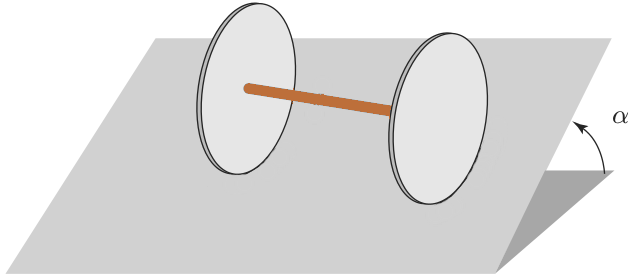
\includegraphics[scale=0.4]{problema1fig1}
 \caption{Representación esquemática del sistema de dos discos que ruedan sin resbalar.}
 \label{fig:problema1fig1}
\end{figure}

Para los discos, el eje puede considerarse como un eje de simetría, y entonces los 
momentos de inercia en el plano de los discos serán iguales $I_1 = I_2 = I$ y a lo 
largo de el eje $\xi\xi'$ será $I_3$. El eje hace un ángulo $\theta$ con la horizontal 
$XX'$. Denotaremos por $\theta$ y $\theta'1$ los ángulos que marcan los puntos de 
referencia de los puntos en la circunferencia de los discos con respecto a la línea 
normal al plano inclinado. Entonces con esas suposiciones y geometría que hemos 
planteado proponemos que podemos describir el sistema en términos de 5 coordenadas 
generalizadas $(X,Y,\theta,\phi,\phi')$. Debajo mostramos el sistema visto de arriba 
para una más fácil visualización de las coordenadas y de los ángulos que hemos 
planteado.

\begin{figure}[H]
 \center
 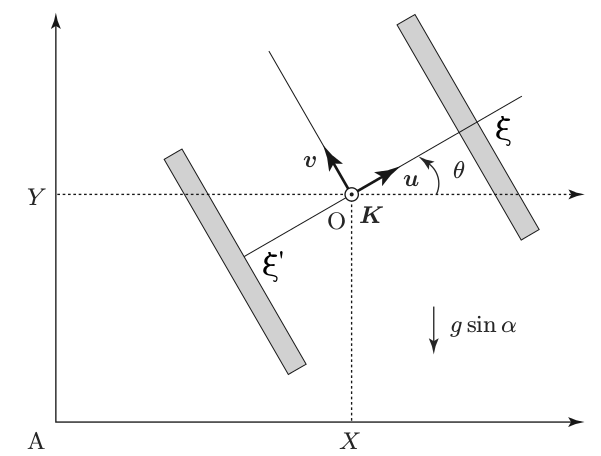
\includegraphics[scale=0.4]{problema1fig2}
 \caption{Geometría del sistema de ejes propuesto sobre el plano inclinado visto desde 
 arriba.}
 \label{fig:problema1fig2}
\end{figure}

Recordamos que el sistema está definido en el plano inclinado, con origen $A$, el eje 
horizontal es $AX$, el eje $AY$ está en la dirección de máximo descenso y $AZ$ es normal 
al plano. Las coordenadas del centro del eje, $O$, las denotaremos por $X$ y $Y$. Sea 
$\mathbf{K}$ el vector unitario normal al plano, $\mathbf{u}$ el vector unitario 
a lo largo de $\mathbf{O\xi}$ y $\mathbf{v}$ el vector unitario del plano perpendicular 
a $\mathbf{O\xi}$. Por esta construcción es fácil ver que $\mathbf{O\xi} = (l/2)\mathbf{u}$.
Debido a que también por construcción $\mathbf{A\xi} = \mathbf{AO} + \mathbf{O\xi}$ la 
velocidad del punto $\xi$ será $\mathbf{V}_\xi = \mathbf{V}_O + (l/2)\dot{\theta}\mathbf{v}$. 
Para obtener las cantidades relativas a $\xi'$ solo bastará con cambiar $l \rightarrow -l$ y 
$\phi \rightarrow \phi'$ a la cantidad relativa a $\xi$ lo cual simplificará 
bastante el trabajo.

\vspace{.3cm}

Debido a que el eje no tiene masa, solo los discos contribuyen a la energía 
cinética. Es fácil ver que el vector de rotación para el disco $\xi$ estará 
dado por $\mathbf{\omega} = \dot{\theta}\mathbf{K} + \dot{\phi}\mathbf{u}$. La 
energía cinética estará dada por la energía del centro de masa de la disco 
más la energía cinética de rotación,

\begin{equation}
 T_\xi = \frac{1}{2}\mathbf{V}_\xi^2 + T_\xi^{(rot)}.
\end{equation}

La energía rotacional se calcula simplemente utilizando $\mathbf{\omega}$ y
los momentos de inercia de los discos, $(T_\xi^{(rot)})_i = I_i(\mathbf{\omega}\cdot \mathbf{\omega})$, 
y ahora usando la expresión para $\mathbf{V}_\xi$ tenemos que 

\begin{equation}
 T_\xi = \frac{1}{2}m\left[\mathbf{V}_O^2 + (l^2/4)\dot{\theta}^2 +
 l\dot{\theta}\mathbf{v}\cdot\mathbf{V}_O \right]
 + \frac{1}{2}\left[ I\dot{\theta}^2 + I_3\dot{\phi}^2\right],
\end{equation}

y para $\xi'$

\begin{equation}
 T_{\xi'} = \frac{1}{2}m\left[\mathbf{V}_O^2 + (l^2/4)\dot{\theta}^2 
 - l\dot{\theta}\mathbf{v}\cdot\mathbf{V}_O \right]
 + \frac{1}{2}\left[ I\dot{\theta}^2 + I_3\dot{\phi}'^2\right].
\end{equation}

Ahora debido a que $\mathbf{V}_O^2 = \dot{X}^2 + \dot{Y}^2$ por la 
construcción que hemos hecho, y sumando las expresiones de las energías 
cinéticas para ambos discos tenemos que,

\begin{align*}
 T &= \frac{1}{2}m\left[(\dot{X}^2 + \dot{Y}^2) + (l^2/4)\dot{\theta}^2 +
 l\dot{\theta}\mathbf{v}\cdot\mathbf{V}_O \right]
 + \frac{1}{2}\left[ I\dot{\theta}^2 + I_3\dot{\phi}^2\right] \\
 %
 &+ \frac{1}{2}m\left[(\dot{X}^2 + \dot{Y}^2) + (l^2/4)\dot{\theta}^2 
 - l\dot{\theta}\mathbf{v}\cdot\mathbf{V}_O \right]
 + \frac{1}{2}\left[ I\dot{\theta}^2 + I_3\dot{\phi}'^2\right], \\
 %
   &= \frac{1}{2}m(\dot{X}^2 + \dot{Y}^2) + \frac{1}{2}m(l^2/4)\dot{\theta}^2 +
      \cancel{\frac{1}{2}ml\dot{\theta}\mathbf{v}\cdot\mathbf{V}_O}
      + \frac{1}{2}I\dot{\theta}^2 + \frac{1}{2}I_3\dot{\phi}^2 \\
  %
  &+ \frac{1}{2}m(\dot{X}^2 + \dot{Y}^2) + \frac{1}{2}m(l^2/4)\dot{\theta}^2 -
      \cancel{\frac{1}{2}ml\dot{\theta}\mathbf{v}\cdot\mathbf{V}_O}
      + \frac{1}{2}I\dot{\theta}^2 + \frac{1}{2}I_3\dot{\phi}'^2,
  %
\end{align*}

\begin{equation}
 \therefore T = m\left(\dot{X}^2 + \dot{Y}^2\right)  
 +\left( I + \frac{1}{4}ml^2 \right) \dot{\theta}^2 
 + \frac{1}{2}I_3 \left(\dot{\phi}^2 + \dot{\phi}'^2\right).
\end{equation}

Veremos que escribir las aceleraciones generalizadas nos será muy útil
para resolver este problema ya que lo haremos utilizando el método de 
los multiplicadores indeterminados de Lagrange. Recordando la expresión
para las aceleraciones generalizadas 

\begin{equation}
 A_i(q,\dot{q},\ddot{q},t) = \frac{d}{dt}\frac{\partial T(q,\dot{q},t)}{\partial\dot{q^i}}
 + \frac{\partial T(q,\dot{q},t)}{\partial q^i},
\end{equation}

tenemos entonces que,

\begin{align}
 A_X &= 2m\ddot{X}, \\
 A_Y &= 2m\ddot{Y}, \\
 A_\theta &= 2 \left( I + \frac{1}{4}ml^2 \right) \ddot{\theta}, \\
 A_\phi &= I_3\ddot{\phi}, \\
 A_{\phi'} &= I_3\ddot{\phi}''.
\end{align}

Necesitamos ahora expresar las condiciones para rodar sin resbalar. Sea 
$\zeta$ el punto de contacto del disco $\xi$con el plano; la condición que 
requerimos es que $\mathbf{V}_\zeta = 0$. Pero sabemos que para $\xi$, 
el vector de rotación instantánea en $\zeta$ puede escribirse como 

\begin{equation}
 \mathbf{V}_\zeta = \mathbf{V}_\xi + \mathbf{\omega}\times \mathbf{\xi\zeta} = 0.
\end{equation}

Esta condición nos dará dos condiciones escalares, lo mismo para 
el disco $\xi'$ que en el punto $\zeta'$ debe cumplirse que 

\begin{equation}
 \mathbf{V}_\zeta' = \mathbf{V}_\xi' + \mathbf{\omega}\times \mathbf{\xi'\zeta'} = 0.
\end{equation}

De estas cuatro condiciones (utilizando la figura \mref{fig:problema1fig2} y la ecuación para $\mathbf{V}_\xi$), 
dos son idénticas, y tenemos entonces tres ecuaciones de constricción,

\begin{align}
 \dot{X}\cos{\theta} + \dot{Y}\sen{\theta} = 0, \\
 \dot{Y}\cos{\theta} - \dot{X}\sen{\theta} + \frac{1}{2}l\dot{\theta} + R\dot{\phi} = 0, \\
 \dot{Y}\cos{\theta} - \dot{X}\sen{\theta} - \frac{1}{2}l\dot{\theta} + R\dot{\phi}' = 0,
\end{align}

Podemos escribir estas ecuaciones de una forma más informativa, haciendo 
un poco de álgebra, como

\begin{align}
\label{eq:discosConstri1}
 2\dot{X} - R (\dot{\phi} + \dot{\phi}')\sen{\theta} = 0, \\
\label{eq:discosConstri2}
 2\dot{Y} + R (\dot{\phi} + \dot{\phi}')\cos{\theta} = 0, \\
\label{eq:discosConstri3}
 l\dot{\theta} + R (\dot{\phi} - \dot{\phi}') = 0.
\end{align}

De estas constricciones, solo \mref{eq:discosConstri3} es holonómica, 
en cambio \mref{eq:discosConstri1} y \mref{eq:discosConstri2} son no holonómicas. 
Estas construcciones representan las constricciones requeridas para rodar 
sin resbalar. 

\vspace{.3cm}

Debido a que los puntos de aplicación para las fuerzas de reacción 
debidos al plano no se desplazan durante un desplazamiento virtual, 
por la condición de rodar sin resbalar, estas fuerzas de reacción no 
implican fuerzas generalizadas. El único trabajo virtual que no 
se hace cero es debido al peso. Podemos calcularla con un desplazamiento 
virtual del centro de masa $O$. Es fácil ver que 

\begin{equation}
 \delta W = - 2mg \delta z_O = -2mg\sen{\alpha}\delta Y,
\end{equation}

entonces la única fuerza generalizada que no se hace cero es 

\begin{equation}
 Q_Y = -2mg\sen{\alpha}.
\end{equation}

Ahora recordando la expresión para el formalismo de los multiplicadores 
indeterminados de Lagrange tenemos que, utilizando las expresiones 
para las aceleraciones generalizadas,

\begin{align}
 m\ddot{X} = \lambda_1, \\
 m\ddot{Y} = - mg\sen{\alpha} + \lambda_2, \\
 2\left( I + \frac{1}{4}ml^2\right) \ddot{\theta} = l\lambda_3, \\
 I_3\ddot{\phi} = -lambda_1 R\sen{\theta} + \lambda_2 R\cos{\theta} + R\lambda_3, \\
 I_3\ddot{\phi}' = -lambda_1 R\sen{\theta} + \lambda_2 R\cos{\theta} - R\lambda_3.
\end{align}


TERMINAR.


\section{Problema 2}

Un sistema consiste de una partícula de masa $m$ en el espacio físico y tiene una 
lagrangiana

$$
L = \frac{1}{2}m(\mathbf{\dot{r}} + \mathbf{\dot{r}}) - V(\mathbf{r}).
$$

La partícula puede describir una trayectoria entre dos puntos $A$ y $B$ en un tiempo 
$t_{AB}$. Demuestre que una partícula de masa $M$ sujeta al mismo potencial podrá 
describir la misma trayectoria entre los puntos $A$ y $B$, pero que el tiempo que 
tardaría sería distinto. Calcule ese tiempo.

\vspace{.3cm}

\underline{Solución:} \vspace{.3cm}

\section{Problema 3}

Una funcional $f(y)$ $(y(t) \in \mathbb{R}^n)$ se define por 

$$
f(y) = \int_{t_{i}}^{t_{f}} F(y,\dot{y},\ddot{y},y)dt.
$$

Encuentre las condiciones o ecuaciones que debe cumplir la curva $y$ para que $f$ sea
extremal cuando fijamos $y(t_i) = y_i$, $y(t_f)=y_f$, $\dot{y}(t_i) = v_i$ y
$\dot{y}(t_f) = v_f$.

\vspace{.3cm}

\underline{Solución:} \vspace{.3cm}

Comencemos calculando la diferencial de la funcional dada, claramente esta debe ser 
diferenciable para poder cumplirse lo que demostraremos en este problema. Usando 
el hecho de 

\begin{equation}
 F(c+h) - F(c) = DF_c[h]+O(|h|^2),
 \label{eq:diferencialFuncional1}
\end{equation}

donde $c$ y $h$ son curvas, y $Df_c$ es una funcional lineal, a la cual se le llama 
la diferencial de la funcional $f$ valuada en la curva $c$, tenemos entonces que, 
donde recordamos que $y = y(t)$, $\dot{y} = \dot{y}(t)$,$\ddot{y} = \ddot{y}(t)$ y $h=h(t)$, 
$\dot{h}=\dot{h}(t)$, $\ddot{h}=\ddot{h}(t)$

\begin{align}
\begin{split}
 f(y+h) - f(y) &= \int_{t_{i}}^{t_{f}} F(y+h,\dot{y}+ \dot{h}, \ddot{y} + \ddot{h}, t)dt -
 \int_{t_{i}}^{t_{f}} F(y,\dot{y},\ddot{y},y)dt, \\
	       &= \int_{t_{i}}^{t_{f}} \left[ F(y+h,\dot{y}+ \dot{h}, \ddot{y} + \ddot{h}, t)
	       -F(y,\dot{y},\ddot{y},y) \right]dt.
 \end{split}
\end{align}

Ahora, como $F$ es una función diferenciable de $\mathbb{R}^{n+n+n+1}$ en $R$ podemos 
escribir, utilizando \mref{eq:diferencialFuncional1}

\begin{equation}
 f(y+h) - f(y) =  \int_{t_{i}}^{t_{f}} \left\{DF_y[h,\dot{h},\ddot{h},t] + O(|h|^2) \right\}dt
\end{equation}

Luego,

\begin{align*}
 f(y+h) - f(y) = \int_{t_{i}}^{t_{f}} \left[ \left\zerodel \sum_{i=1}^n  \left( \frac{\partial F}{\partial y_i}h_i + 
 \frac{\partial F}{\partial \dot{y}_i}\dot{h}_i + \frac{\partial F}{\partial \ddot{y}_i}\ddot{h}_i\right)\right|_{y} 
 + O(|h|^2) \right]dt, \\
%  
	      = \sum_{i=1}^n \left[\int_{t_{i}}^{t_{f}}\left\zerodel\frac{\partial F}{\partial y_i}\right|_y h_i dt  
	      + \int_{t_{i}}^{t_{f}} \left\zerodel\frac{\partial F}{\partial \dot{y}_i}\right|_y \dot{h}_i dt
	       + \int_{t_{i}}^{t_{f}} \left\zerodel\frac{\partial F}{\partial \ddot{y}_i}\right|_y \ddot{h}_i dt\right] 
	       +  \int_{t_{i}}^{t_{f}} O(|h|^2)dt
 %
\end{align*}

Integrando por parte el segundo y el primer término tenemos que

\begin{equation}
  \int_{t_{i}}^{t_{f}} \left\zerodel\frac{\partial F}{\partial \dot{y}_i}\right|_y \dot{h}_i dt = 
  - \int_{t_{i}}^{t_{f}} \frac{d}{dt}\left(\left\zerodel\frac{\partial F}{\partial \dot{y}}\right)\right|_y h_i dt + 
  \left\zerodel\frac{\partial F}{\partial \dot{y}}\right|_y \left\zerodel h_i\right|_{t_{i}}^{t_{f}},
\end{equation}

y

\begin{equation}
  \int_{t_{i}}^{t_{f}} \left\zerodel\frac{\partial F}{\partial \ddot{y}_i}\right|_y \ddot{h}_i dt = 
  - \int_{t_{i}}^{t_{f}} \frac{d}{dt}\left(\left\zerodel\frac{\partial F}{\partial \ddot{y}}\right)\right|_y \dot{h}_i dt + 
  \left\zerodel\frac{\partial F}{\partial \ddot{y}}\right|_y \left\zerodel \dot{h}_i\right|_{t_{i}}^{t_{f}},
\end{equation}

Entonces tenemos que,

\begin{align}
 \begin{split}
  f(y+h) - f(y) =  &\sum_{i=1}^n \left[\int_{t_{i}}^{t_{f}}\left\zerodel\frac{\partial F}{\partial y_i}\right|_y h_i dt 
   - \int_{t_{i}}^{t_{f}} \frac{d}{dt}\left(\left\zerodel\frac{\partial F}{\partial \dot{y}}\right)\right|_y h_i dt + 
  \left\zerodel\frac{\partial F}{\partial \dot{y}}\right|_y \left\zerodel h_i\right|_{t_{i}}^{t_{f}}\right\zerodel \\
  %
  &- \left\zerodel\int_{t_{i}}^{t_{f}} \frac{d}{dt}\left(\left\zerodel\frac{\partial F}{\partial \ddot{y}}\right)\right|_y \dot{h}_i dt + 
  \left\zerodel\frac{\partial F}{\partial \ddot{y}}\right|_y \left\zerodel \dot{h}_i\right|_{t_{i}}^{t_{f}}\right]
  +  \int_{t_{i}}^{t_{f}} O(|h|^2)dt \\
  %
  &= \sum_{i=1}^n\left[\int_{t_{i}}^{t_{f}}\left\zerodel\frac{\partial F}{\partial y_i}\right|_y h_i dt 
   - \int_{t_{i}}^{t_{f}} \frac{d}{dt}\left(\left\zerodel\frac{\partial F}{\partial \dot{y}}\right)\right|_y h_i dt + 
  \left\zerodel\frac{\partial F}{\partial \dot{y}}\right|_y \left\zerodel h_i\right|_{t_{i}}^{t_{f}}\right\zerodel \\
  %
  &-\left\zerodel \int_{t_{i}}^{t_{f}} \frac{d^2}{dt^2}\left(\left\zerodel\frac{\partial F}{\partial \ddot{y}}\right)\right|_y h_i dt + 
  \left\zerodel\frac{\partial F}{\partial \ddot{y}}\right|_y \left\zerodel \dot{h}_i\right|_{t_{i}}^{t_{f}}\right]
  +  \int_{t_{i}}^{t_{f}} O(|h|^2)dt
  %
 \end{split}
\end{align}

Tenemos entonces que 

\begin{align*}
 f(y+h) - f(y) &= \sum_{i=1}^n \int_{t_{i}}^{t_{f}} \left[\frac{\partial F}{\partial y_i}  - 
 \frac{d}{dt}\frac{\partial F}{\partial \dot{y}}  
 - \frac{d^2}{dt^2}\frac{\partial F}{\partial \ddot{y}} \right]_y h_i dt \\
 &+\sum_{i=1}^n \left\zerodel \left\zerodel\frac{\partial F}{\partial \dot{y}}\right|_y h_i\right|_{t_{i}}^{t_{f}}
 + \sum_{i=1}^n \left\zerodel \left\zerodel\frac{\partial F}{\partial \ddot{y}}\right|_y\dot{h}_i\right|_{t_{i}}^{t_{f}}
 + \int_{t_{i}}^{t_{f}} O(|h|^2)dt
\end{align*}

Tenemos entonces que la diferencial está dada por

\begin{align}
\begin{split}
 DF_c[h] &=  \sum_{i=1}^n \int_{t_{i}}^{t_{f}} \left[\frac{\partial F}{\partial y_i}  - 
 \frac{d}{dt}\frac{\partial F}{\partial \dot{y}}  
 - \frac{d^2}{dt^2}\frac{\partial F}{\partial \ddot{y}} \right]_y h_i dt \\
 &+\sum_{i=1}^n \left\zerodel \left\zerodel\frac{\partial F}{\partial \dot{y}}\right|_y h_i\right|_{t_{i}}^{t_{f}}
 + \sum_{i=1}^n \left\zerodel \left\zerodel\frac{\partial F}{\partial \ddot{y}}\right|_y\dot{h}_i\right|_{t_{i}}^{t_{f}}
 \end{split}
 \label{eq:diferencialFuncional2}
\end{align}


Para resolver este problema, limitamos las posibles curvas a aquellas que 
para pasan por puntos fijos, y que cumplen con las condiciones del enunciado, con lo 
cual vemos que la variación de $h_i$ y $\dot{h}_i$ es cero evaluada entre $t_i$ y $t_f$, 
haciendo cero a los dos últimos términos de \mref{eq:diferencialFuncional2}, y entonces 
como el resto de las cantidades dentro del primer término de \mref{eq:diferencialFuncional2}
son independientes de $h(t)$, para que se cumpla que la curva $y$ para que $f$ sea 
extremal debe cumplirse que 

\begin{equation}
\boxed{\frac{\partial F}{\partial y_i}  - 
 \frac{d}{dt}\frac{\partial F}{\partial \dot{y}}  
 - \frac{d^2}{dt^2}\frac{\partial F}{\partial \ddot{y}} = 0.}
 \label{eq:condicionExtremal}
\end{equation}

Decimos entonces que la funcional $f$, y dentro del espacio de las curvas que pasan 
por un punto específico para $t=t_0$ y por otro para $t=t_1$, las curvas para que la 
funcional tiene una extremal están dadas por las ecuaciones \mref{eq:condicionExtremal}.



\section{Problema 4}

Demuestre que la formulación lagrangiana de la mecánica es invariante ante el grupo 
de Galileo.

\vspace{.3cm}

\underline{Solución:} \vspace{.3cm}

\section{Problema 5}

Demuestre, con toda formalidad y usando el teorema de Noether, que la lagrangiana 
de una partícula libre en tres dimensiones es invariante ante el grupo de rotaciones 
$SO(3)$ y que por ello se conserva el vector de impulso angular.

\vspace{.3cm}

\underline{Solución:} \vspace{.3cm}

\section{Problema 6}

En el caso de una dependencia explícita del tiempo se utiliza una variedad de configuración 
extendida para tratar el teorema de Noether. En esta variedad se utiliza una lagrangiana 
extendida de la formalidad

$$
L_{ext} = L(q,\frac{\overline{q}}{\overline{t}})\overline{t},
$$

donde $L$ es la lagrangiana del sistema. ¿Cuál es la razón de utilizar esta forma y no 
otra que también se redujera a la lagrangiana del sistema cuando $\overline{t}=1$?

\vspace{.3cm}

\underline{Solución:} \vspace{.3cm}

\begin{thebibliography}{20}
\bibitem{ginoux}
C. Ginoux y B. Silvestre-Brac,\emph{Solved Problems in Lagrangian and Hamiltonian Mechanics},
Springer, 2009.
\end{thebibliography}


\end{document}
